\pagebreak
\section{Enhanced Entity Relationship Model (EER)}
\begin{figure}[h!]
\centering
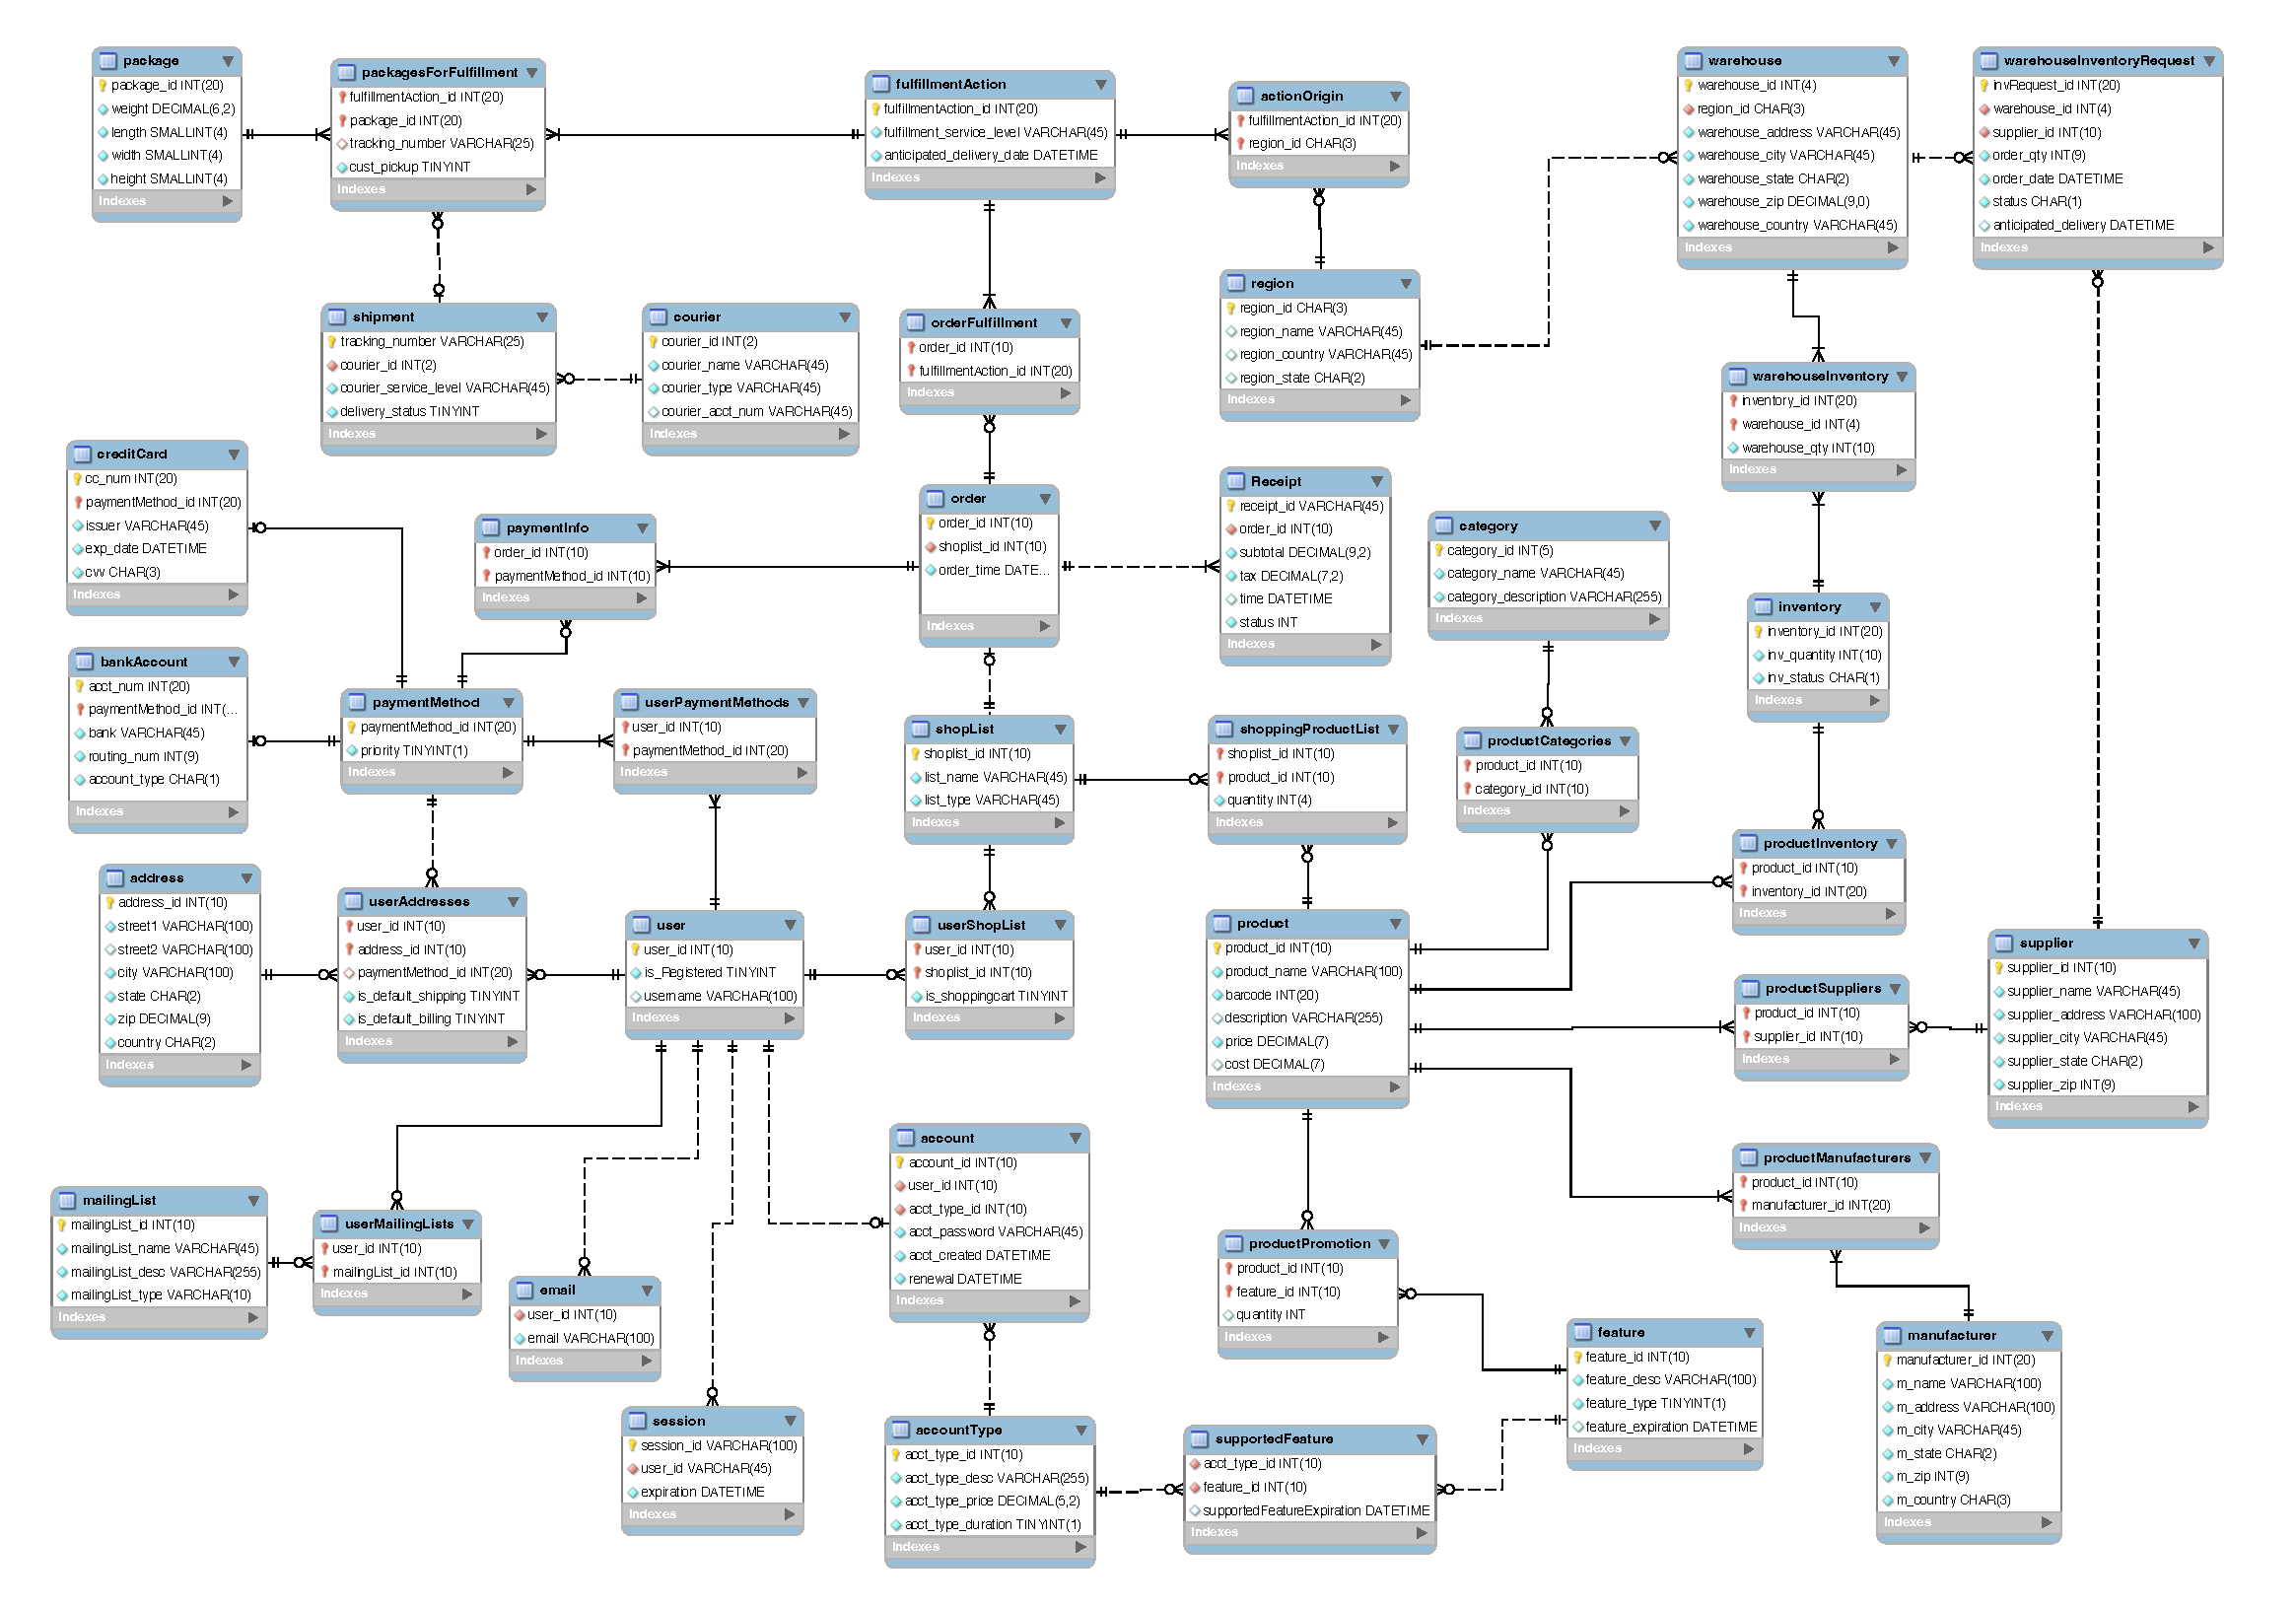
\includegraphics[scale= 0.511, angle=90]{EER.pdf}
\caption{EER Diagram}
\end{figure}

\begin{spacing}{1.25}
\begin{longtable}{ | p{0.25\linewidth} | p{0.15\linewidth} | p{0.126\linewidth} | p{0.128\linewidth} | p{0.22\linewidth} | }
\caption{Implementation for Foreign Keys}\\
\hline
Table						& FK 				& ON DELETE & ON UPDATE & Comments\\\hline\endhead
packagesForFulfillment 		& fulfillmentAction	& CASCADE 	& CASCADE 	& If a fulfillment action is deleted/updated, then the packages for fulfillment should be deleted/updated as well\\\hline
packagesForFulfillment 		& package 			& CASCADE 	& CASCADE 	& If a package is deleted/updated, then the packages for fulfillment should be deleted/updated as well\\\hline
packagesForFulfillment	 	& shipment 			& SET NULL 	& CASCADE 	& If a shipment is updated, then the packages for fulfillment should be updated as well. If a shipment is deleted, then the shipment info in packagesForFulfillment should be set to null and cust\_pickup flag set to true; this is the case where the customer chooses to pick up the order at the warehouse.\\\hline
actionOrigin		 		& fulfillmentAction	& CASCADE 	& CASCADE 	& If a fulfillment action is deleted/updated, then the action origin should be deleted/updated as well\\\hline
actionOrigin		 		& region 			& RESTRICT 	& RESTRICT 	& A region should be restricted from deletion/update since the action is non-trivial.  Otherwise, many fulfillment actions associated with a particular region will end up being orphaned or changed to a region that may not be appropriate for the action.  Hence, deletion/update of a region should only occur when there is a new region that can replace it or if the region still overlaps with the previous scope.\\\hline
warehouse			 		& region			& RESTRICT 	& RESTRICT 	& A region should be restricted from deletion/update since the action is non-trivial. Deletion/update of a region should only occur when there is a new region that can replace it or if the region still overlaps with the previous version.  Otherwise, warehouses would end up being deleted/updated along with the region. Because they are physical spaces, they cannot move if the scope of a region is changed.\\\hline
warehouseInventoryRequest	& warehouse			& CASCADE 	& CASCADE 	& A deletion/update of a warehouse should delete/update an inventory request.\\\hline
warehouseInventoryRequest	& supplier			& CASCADE 	& CASCADE 	& A deletion/update of a supplier should delete/update an inventory request.\\\hline
warehouseInventory			& inventory			& CASCADE 	& CASCADE 	& A deletion/update of an inventory should delete/update a warehouse inventory.\\\hline
warehouseInventory			& warehouse			& CASCADE 	& CASCADE 	& A deletion/update of a warehouse should delete/update a warehouse inventory.\\\hline
receipt						& orderDetails		& CASCADE	& CASCADE 	& A deletion/update of an order should delete/update a receipt.\\\hline
orderFulfillment			& orderDetails		& CASCADE	& CASCADE 	& A deletion/update of an order should delete/update an order fulfillment.\\\hline
orderFulfillment			& fulfillmentAction	& CASCADE	& CASCADE 	& A deletion/update of a fulfillment action should delete/update an order fulfillment.\\\hline
shipment					& courier			& RESTRICT	& CASCADE 	& A deletion of a courier should be restricted since many shipments are associated with a particular courier.  Deletion of a courier should only occur if a replacement courier has already been considered for all shipments associated with the courier.  An update of a courier should update a shipment.\\\hline
creditCard					& paymentMethod		& CASCADE	& CASCADE 	& A deletion/update of the payment method should delete/update the credit card.\\\hline
bankAccount					& paymentMethod		& CASCADE	& CASCADE 	& A deletion/update of the payment method should delete/update the bank account.\\\hline
paymentInfo					& orderDetails		& CASCADE	& CASCADE 	& A deletion/update of an order should delete/update the payment information.\\\hline
paymentInfo					& paymentMethod		& CASCADE	& CASCADE 	& A deletion/update of a payment method should delete/update the payment information.\\\hline
orderDetails				& shopList			& CASCADE	& CASCADE 	& A deletion/update of a shopping list should delete/update the order.\\\hline
productCategories			& product			& CASCADE	& CASCADE 	& A deletion/update of a product should delete/update the product categories.\\\hline
productCategories			& category			& CASCADE	& CASCADE 	& A deletion/update of a category should delete/update the product categories.\\\hline
shoppingProductList			& shopList			& CASCADE	& CASCADE 	& A deletion/update of a shopList should delete/update the shopping product list.\\\hline
shoppingProductList			& product			& CASCADE	& CASCADE 	& A deletion/update of a product should delete/update the shopping product list.\\\hline
userPaymentMethods			& user				& CASCADE	& CASCADE 	& A deletion/update of a user should delete/update the user payment method.\\\hline
userPaymentMethods			& paymentMethod		& CASCADE	& CASCADE 	& A deletion/update of a paymentMethod should delete/update the user payment method.\\\hline
userAddresses				& user				& CASCADE	& CASCADE 	& A deletion/update of a user should delete/update the user addresses.\\\hline
userAddresses				& address			& CASCADE	& CASCADE 	& A deletion/update of an address should delete/update the user addresses.\\\hline
userShopList				& user				& CASCADE	& CASCADE 	& A deletion/update of a user should delete/update the user shop list.\\\hline
userShopList				& shoplist			& CASCADE	& CASCADE 	& A deletion/update of a shopping list should delete/update the user shop list.\\\hline
productInventory			& product			& RESTRICT	& CASCADE 	& The deletion of a product should be restricted since the existence of inventory implies the existence of a product; deletion should only occur if there is no more product inventory.  An update of a product should update the product inventory.\\\hline
productInventory			& inventory			& CASCADE	& CASCADE 	& A deletion/update of an inventory item should delete/update the product inventory.\\\hline
productSuppliers			& product			& CASCADE	& CASCADE 	& A deletion/update of a product should delete/update the product supplier.\\\hline
productSuppliers			& supplier			& CASCADE	& CASCADE 	& A deletion/update of a supplier should delete/update the product supplier.\\\hline
productManufacturers		& product			& CASCADE	& CASCADE 	& A deletion/update of a product should delete/update the product manufacturer.\\\hline
productManufacturers		& manufacturer		& CASCADE	& CASCADE 	& A deletion/update of a manufacturer should delete/update the product manufacturer.\\\hline
productPromotion			& product			& CASCADE	& CASCADE 	& A deletion/update of a product should delete/update the product promotion.\\\hline
productPromotion			& feature			& CASCADE	& CASCADE 	& A deletion/update of a feature should delete/update the product promotion.\\\hline
supportedFeature			& accountType		& CASCADE	& CASCADE 	& A deletion/update of an account type should delete/update the supported feature.\\\hline
supportedFeature			& feature			& CASCADE	& CASCADE 	& A deletion/update of a feature should delete/update the supported feature.\\\hline
account						& user				& CASCADE	& CASCADE 	& A deletion/update of a user should delete/update the account.\\\hline
account						& accountType		& RESTRICT	& CASCADE 	& The deletion of an accountType should be restricted since such a deletion would delete many accounts. Deletion should only occur if there does not exist accounts of the account type. An update of an accountType should update the account.\\\hline
session						& user				& CASCADE	& CASCADE 	& A deletion/update of a user should delete/update the session.\\\hline
email						& user				& CASCADE	& CASCADE 	& A deletion/update of a user should delete/update the email.\\\hline
userMailingLists			& user				& CASCADE	& CASCADE 	& A deletion/update of a user should delete/update the user mailing lists.\\\hline
userMailingLists			& mailingList		& CASCADE	& CASCADE 	& A deletion/update of a mailing list should delete/update the user mailing lists.\\\hline
\end{longtable}
\end{spacing}